\section{Camera fundamenals}
A gentle introduction to the pinhole camera model, projection matrix, calibration (internal and external), the underlying mathematics.

\begin{figure}[hbt!]
	\centering
	%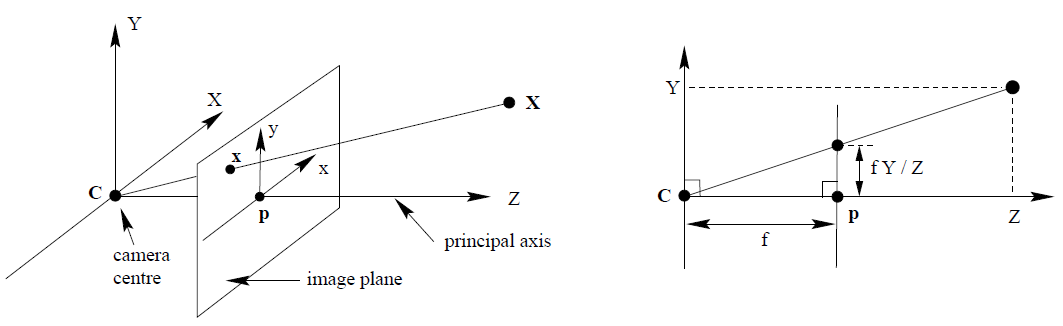
\includegraphics[width=\linewidth]{perspective_projection_3.png}
	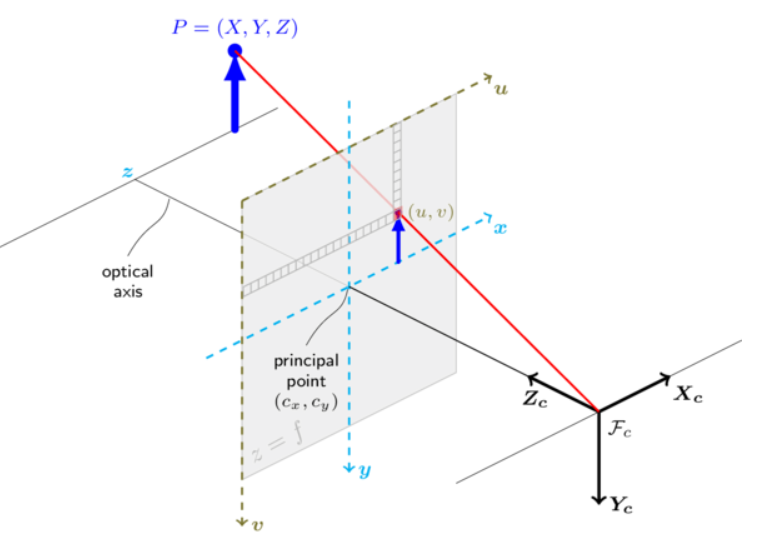
\includegraphics[scale=0.5]{perspective_projection_4.png}
	\caption{Pinhole camera geometry. $\vect{F_c}$ \textit{is the camera center,} \textbf{$(C_x, C_y)$} \textit{is the principal point,} $\vect{P}$ \((X, Y, Z)^T\)  \textit{is world point,} $\vect{P_c}$ \((X_c, Y_c, Z_c)^T\) \textit{is world point measured in camera coordinate system.\cite{OpenCV}} }
	\label{fig:perspective projection}
\end{figure}

A simplified perspective projection is shown in \cref{fig:perspective projection}. A world point \( \displaystyle (X_c, Y_c, Z_c)^T\)  is mapped to \( ( \textit{f}\frac{X_c}{Z_c}, \textit{f}\frac{Y_c}{Z_c}, \textit{f} )^T \) on the image plane placed at a focal length distance \textit{f} from the camera center $(F_c)$. Two key facts can be derived from the above projection equation that farther the object is (larger the $Z_c$) from the camera, smaller the size in image plane (shrinking operation) and these shrunk points are magnified by the focal length \textit{f} to be placed on the image plane. World points are first shrunk \( (x, y)^T =  (\frac{X_c}{Z_c}, \frac{Y_c}{Z_c})^T \) and then magnified \( ( \textit{f}\frac{X_c}{Z_c}, \textit{f}\frac{Y_c}{Z_c}, \textit{f} )^T.\)

Often, the world points are represented in homogeneous coordinates due to several advantages, being able to express infinite quantities is one of them. The linear mapping between world and image points is evident in the homogeneous representation as shown below.\\ 

\begin{equation}
Z_c \left[
\begin{array}{c} x\\ y\\ 1 \end{array} 
\right] = 
\begin{bmatrix}
\textit{f} & 0 & 0 & 0 \\
0 & \textit{f} & 0 & 0 \\
0 & 0 & 1 & 0
\end{bmatrix} 
\left[
\begin{array}{c} X_c\\ Y_c\\ Z_c\\ 1 \end{array} 
\right]
\label{eq:mat_image_t_camera}
\end{equation}

The linear mapping can be expressed in a compact form $ \vect{x} = \matr{P} \vect{X_c} $ where $\vect{x}$ is a vector of image points, $\vect{X}$ is a vector of world points and $\matr{P}$ is a 3x4 homogeneous matrix called camera projection matrix. In general, the origin of the image plane may not coincide with the principal point, therefore it is necessary to map the projected points to pixels before using the image for further use as show in \cref{fig:mm_to_pixel}.

\begin{figure}[hbt!]
	\centering
	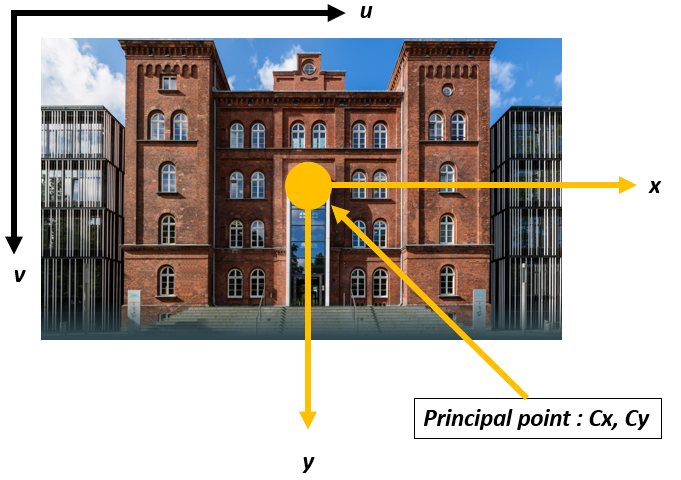
\includegraphics[width=\linewidth]{mm_to_pixel.png}
	\caption{Pixel coordinates $(u,v)$ and the camera coordinates $(x, y)$.}
	\label{fig:mm_to_pixel}
\end{figure}

The equation \ref{eq:mm_to_pixel} depicts mapping image to pixel coordinates. wehere $(S_x)$ is size of pixel width and  $(S_y)$ is size of pixel height. \\
\begin{equation}
\begin{split}
(u-C_x) = \frac{x}{S_x}\\
(v-C_y) = \frac{y}{S_y}
\label{eq:mm_to_pixel}
\end{split}
\end{equation}

Therefore a 3D world point \((X_c, Y_c, Z_C)^T\) is mapped to \( ( \textit{f}\frac{X}{Z}+C_x, \textit{f}\frac{Y}{Z}+C_y, \textit{f} )^T \) to the pixel coordinates \( (u, v, z) \) and can be expressed as a matrix multiplication. Where $\alpha_x$ is $(\frac{\textit{f}}{S_x})$ , $\alpha_y$ is $(\frac{\textit{f}}{S_y})$ and S' is slant factor, when the image plane is not normal to the optical axis.

\begin{equation}
\left[ 
\begin{array}{c} u\\ v\\ 1 \end{array} 
\right] = 
\begin{bmatrix}
\frac{1}{S_x} & S' & C_x \\
0 & \frac{1}{S_y} & C_y \\
0 & 0 & 1
\end{bmatrix} 
\left[ 
\begin{array}{c} x\\ y\\ z \end{array} 
\right]
\label{eq:mat_pixel_t_image}
\end{equation}

\begin{equation}
Z_c \left[ 
\begin{array}{c} u\\ v\\ 1 \end{array} 
\right] = 
\begin{bmatrix}
\alpha_x & S & C_x \\
0 & \alpha_y & C_y \\
0 & 0 & 1
\end{bmatrix} 
\begin{bmatrix}
1 & 0 & 0 & 0 \\
0 & 1 & 0 & 0 \\
0 & 0 & 1 & 0
\end{bmatrix}
\left[ 
\begin{array}{c} X_c\\ Y_c\\ Z_c\\ 1 \end{array} 
\right]
\label{eq:mat_pixel_t_camera}
\end{equation}

\begin{equation}
Z_c \left[ 
\begin{array}{c} u\\ v\\ 1 \end{array} 
\right] = 
\left[ 
\begin{array}{c} K_{3\times3} \end{array} 
\right] 
\left[ 
\begin{array}{c} I_{3\times3} | 0 \end{array} 
\right]
\left[ 
\begin{array}{c} X_c\\ Y_c\\ Z_c\\ 1 \end{array}
\right]
\label{eq:_mat_camera_instrinsic}
\end{equation}

In summary, the equation \ref{eq:mat_image_t_camera} maps the world point measured in camera coordinates to image coordinates while equation \ref{eq:mat_pixel_t_image} converts these image coordinates to pixel coordinates. Overall mapping from camera coordinates to the pixel coordinates is depicted in the equation \ref{eq:mat_pixel_t_camera}. K in equation \ref{eq:_mat_camera_instrinsic} is known as the camera intrinsic matrix and depends only on the internals of the camera. In general, a 3D world point \( (X, Y, Z)^T \) may not be known in the camera coordinate system however it can be mapped using 4$\times$4 homogeneous transformation matrix. equation \ref{eq:mat_pixel_t_world} is a mapping from a 3D world point to pixel coordinates. The 4$\times$4 homogeneous transformation matrix is known as an extrinsic matrix and describes the position and orientation of the 3D world point in the camera coordinate system.

\begin{equation}
Z_c \left[ 
\begin{array}{c} u\\ v\\ 1 \end{array} 
\right] = 
\begin{bmatrix}
\alpha_x & S & C_x \\
0 & \alpha_y & C_y \\
0 & 0 & 1
\end{bmatrix} 
\begin{bmatrix}
r_{11} &r_{12}  &r_{13}  &t_x\\
r_{21} &r_{22}  &r_{23}  &t_y\\
r_{31} &r_{32}  &r_{33}  &t_z \\
0 &0  &0  &1
\end{bmatrix}
\left[ 
\begin{array}{c} X\\ Y\\ Z\\ 1 \end{array} 
\right]
\label{eq:mat_pixel_t_world}
\end{equation}

The equation \ref{eq:mat_pixel_t_world} can be compactly written by combining both intrinsic and extrinsic matrix known as the projection matrix \textbf{$P_{3X4}$}. Where P = K[R|t], and $\lambda$ is a arbitrary scaling factor for which equation \ref{eq:mat_projection} is satisfied.

\begin{equation}
\lambda \left[ 
\begin{array}{c} u\\ v\\ 1 \end{array} 
\right] = 
\begin{bmatrix}
p_{11} &p_{12}  &p_{13}  &p_{14}\\
p_{21} &r_{22}  &r_{23}  &p_{24}\\
p_{31} &p_{32}  &p_{33}  &p_{34} \\
\end{bmatrix}
\left[ 
\begin{array}{c} X\\ Y\\ Z\\ 1 \end{array} 
\right]
\label{eq:mat_projection}
\end{equation} 
We extract the camera center from the projection matrix as the camera center C = $-\inv{R}t$ or in other words, $t = -RC$. Therefore the projection matrix can be written as,
\begin{equation}
\begin{split}
	\matr{P} = \matr{K}\ [\matr{R}\ |\ \vect{t}]\\
	  = \matr{K}\matr{R}\ [\matr{I}\ |\ -\vect{C}]\\
      = \matr{M}\ [\matr{I}\ |\ \invMat{M}\ \textbf{$p_4$}]
\end{split}
\label{eq:projection_split_up}
\end{equation}
where M = KR, K is a 3x3 upper triangular camera matrix, R is a 3x3 rotation matrix and $p_4$ is the last column of the projection matrix.

\section{Camera calibration}
Often in practice, estimating intrinsic and extrinsic parameters are important and there are many ways to do so. Two approaches will be presented here, one using projection matrix from equation \ref{eq:mat_projection} (2D/3D correspondence) and using homography (2D/2D correspondence).

\subsection{2D/3D correspondence}

\begin{figure}[hbt!]
	\centering
	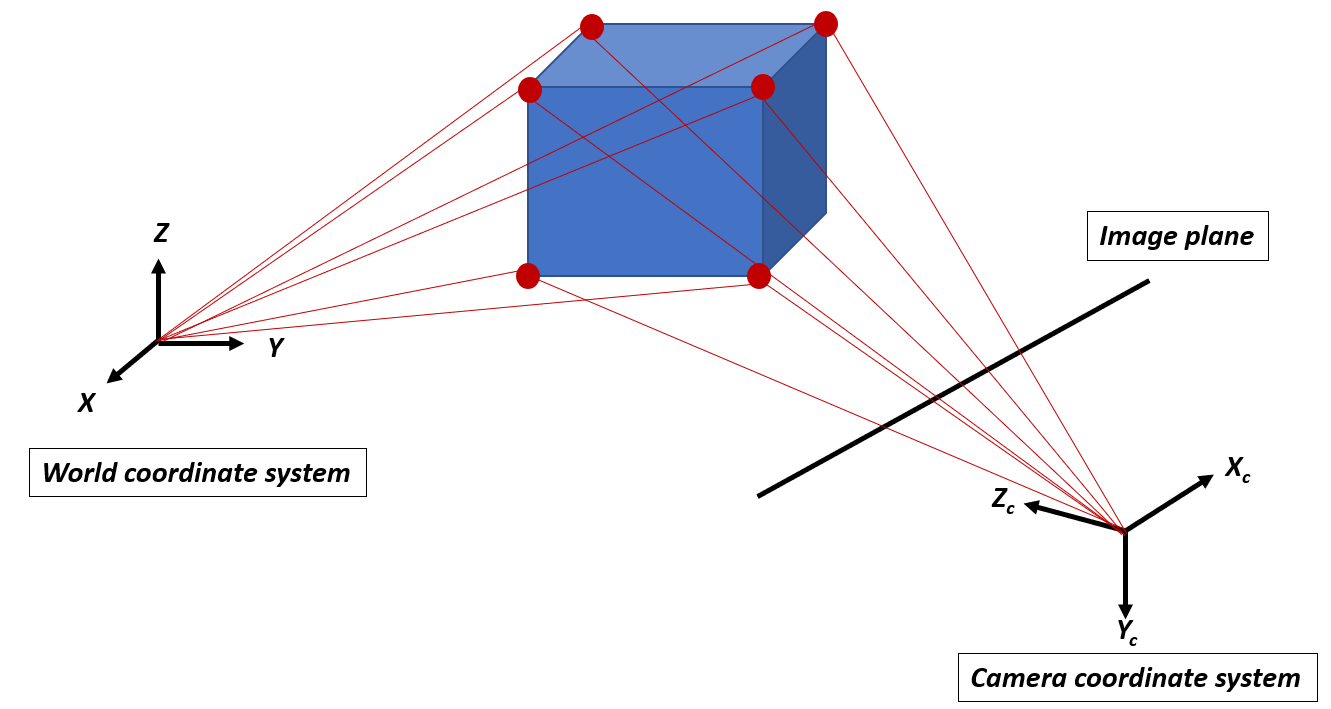
\includegraphics[width=\linewidth]{2D_3D.png}
	\caption{Mapping 3D world points on to a 2D image plane.}
	\label{fig:2D_3D}
\end{figure}

The \cref{fig:2D_3D} depicts a 2D image of a 3D object with known 6 unique points. Recall  the equation \ref{eq:mat_projection} projection matrix P maps the world point to pixel coordinates and the equation is valid for arbitrary scaling factor $\lambda$. First, the projection matrix P will be estimated using a given set of 3D world points and 2D image points and then it will be decomposed to intrinsic and extrinsic matrices as P = K[R|t]. The first step in estimating projection matrix is to convert the equation \ref{eq:mat_projection} into least square problem of type II (see appendix) Ap = 0 subjected to $ \|p\| = 1 $ and solve for vector $\vect{p}$ which is reshaped version of non-trivial elements of the projection matrix P. 

Given a set of N corresponding 2D/3D points (\textbf{$u_i$},\textbf{$X_i$}), a projection matrix P is needed such that

\begin{equation*}
	\lambda\textbf{$u_i$} = P \textbf{$X_i$}\ ,  where\ i = 1......N
\end{equation*}
since the scaling factor $\lambda$ is unknown and has to be estimated while estimating P. we will make use of DLT (direct linear transformation) to convert the above equation to the form Ap = 0.

\begin{equation*}
\left[ 
\begin{array}{c} \lambda u_i\\ \lambda v_i\\ \lambda  \end{array} 
\right] = 
\begin{bmatrix}
p_{11} &p_{12}  &p_{13}  &p_{14}\\
p_{21} &r_{22}  &r_{23}  &p_{24}\\
p_{31} &p_{32}  &p_{33}  &p_{34} \\
\end{bmatrix}
\left[ 
\begin{array}{c} X_i\\ Y_i\\ Z_i\\ 1 \end{array} 
\right]
\end{equation*} 

extracting the bottom row, equation for $\lambda$ and substituting $\lambda$ in other 2 rows yileds
\begin{equation*}
\lambda = p_{31}\textbf{$X_i$} + p_{32}\textbf{$Y_i$} + p_{33}\textbf{$Z_i$} + p_{34}
\end{equation*}

\begin{equation*}
\begin{split}
\textbf{$u_i$}\lambda = \textbf{$u_i$} (p_{31}\textbf{$X_i$} + p_{32}\textbf{$Y_i$} +  p_{33}\textbf{$Z_i$} + p_{34}) = p_{11}\textbf{$X_i$} + p_{12}\textbf{$Y_i$} + p_{13}\textbf{$Z_i$} + p_{14}\\
\textbf{$v_i$}\lambda = \textbf{$v_i$} (p_{31}\textbf{$X_i$} + p_{32}\textbf{$Y_i$} +  p_{33}\textbf{$Z_i$} + p_{34}) = p_{21}\textbf{$X_i$} + p_{22}\textbf{$Y_i$} + p_{23}\textbf{$Z_i$} + p_{24}
\end{split}
\end{equation*}
Rearrangement of the above equations leads to a linear system of equations with non-trivial elements of the projection matrix being reshaped into a vector $\vect{p}$.   

\begin{equation}
\begin{bmatrix}
\textbf{$X_i$} & \textbf{$Y_i$} & \textbf{$Z_i$} & 1 & 0 & 0 & 0 & 0 & \textbf{$-u_i X_i$} & \textbf{$-u_iY_i$} & \textbf{$-u_i Z_i$} & -u_i\\
0 & 0 & 0 & 0 & \textbf{$X_i$} & \textbf{$Y_i$}  & \textbf{$Z_i$} & 1 & \textbf{$-v_iX_i$} & \textbf{$-v_iY_i$} & \textbf{$-v_iZ_i$} & -v_i
\end{bmatrix}
\textbf{p} = \textbf{0}
\label{eq:mat_projection_1}
\end{equation} 

\begin{equation*}
with\ \textbf{p} = \left (p_{11}, p_{12}.........p_{33},p_{34})^T  \in \mathcal{R}^{12} \right. 
\end{equation*}
A projection matrix has 12 non-trivial elements thus 11 degrees of freedom (ignoring scaling) therefore it is necessary to have 11 equations to solve for P. Each pair of 2D/3D point correspondences leads to 2 equations thus a minimum of 6 2D/3D point correspondences are required. Stacking these 6 equations along rows leads to a linear system of equations Ap=0 as shown in \cref{eq:mat_projection_final}. 
\begin{equation}
\begin{bmatrix}
\textbf{$X_1$} & \textbf{$Y_1$} & \textbf{$Z_1$} & 1 & 0 & 0 & 0 & 0 & \textbf{$-u_1 X_1$} & \textbf{$-u_1Y_1$} & \textbf{$-u_1 Z_1$} & -u_1\\
0 & 0 & 0 & 0 & \textbf{$X_1$} & \textbf{$Y_1$}  & \textbf{$Z_1$} & 1 & \textbf{$-v_1X_1$} & \textbf{$-v_1Y_1$} & \textbf{$-v_1Z_1$} & -v_1\\
\vdots & \vdots  & \vdots  & \vdots  & \vdots  & \vdots  & \vdots  & \vdots  & \vdots  & \vdots  & \vdots  & \vdots\\
\textbf{$X_6$} & \textbf{$Y_6$} & \textbf{$Z_6$} & 1 & 0 & 0 & 0 & 0 & \textbf{$-u_6 X_6$} & \textbf{$-u_6Y_6$} & \textbf{$-u_6 Z_6$} & -u_6\\
0 & 0 & 0 & 0 & \textbf{$X_6$} & \textbf{$Y_6$}  & \textbf{$Z_6$} & 1 & \textbf{$-v_6X_i$} & \textbf{$-v_6Y_6$} & \textbf{$-v_6Z_6$} & -v_6\\
\end{bmatrix}
\textbf{p} = \textbf{0}
\label{eq:mat_projection_final}
\end{equation} 

\textbf{Exact solution.} With a minimum of 6 correspondences, the solution to \ref{eq:mat_projection_final} will be exact which means 3D world points will be exactly gets projected to their measured image points correspondingly. The exact solution p, to Ap = 0 is the right nullspace of matrix A.\\

\textbf{Over-determined solution.} Practical measurements will be noisy due to various reasons and therefore we may require more than 6 2D/3D correspondences. In this case, the solution to Ap = 0 will be obtained by minimizing the algebraic or geometric error of projection, subjected to some valid constraints.\\ 

\textbf{Minimizing algebraic error.} In this case the approach is,   

\begin{equation}
\begin{matrix}
\displaystyle \min & \|Ap\| & \textrm{s.t.} & \|p\| = 1\\
\end{matrix}
\label{eq:min_algebraic}
\end{equation}
The solution to \cref{eq:min_algebraic} is obtained from unit singular value of A corresponding to the smallest singular value (the least square problem of type II, see appendix).\\

\textbf{Minimizing geometric error.} First let us define what is geometric error. Let us recall \cref{eq:mat_projection}, \textbf{$u_i$} = P\textbf{$X_i$}, suppose we know 3D world points \textbf{$X_i$} far more accurately than the measured image points then the geometric error in the image is 
\begin{equation*}
\begin{matrix}
\displaystyle \sum_{i=1}^{n} d (u_i, \hat{u}_i)^2 
\end{matrix}
\end{equation*}
where $u_i$ is measured point in the image and $\hat{u}_i$ is P \textbf{$X_i$} which is the exact projection of \textbf{$X_i$} on to the image under P. If the measurement errors are Gaussian then the solution to 
\begin{equation}
\begin{matrix}
\displaystyle \min_{P} \sum_{i=1}^{n} d (u_i, P\textbf{$X_i$})^2 
\end{matrix}
\label{eq:min_geometric}
\end{equation}

is the maximum likelihood of P  as per \cite{Hartley:2003:MVG:861369}. Minimizing geometric error requires non-linear iterative methods such as Levenberg-Marquardt (LM) algorithms. Local minima can be found via LM, in order to find the global minima, the initial starting point can be linear solution obtained from \cref{eq:min_algebraic}.\\

Having estimated projection matrix task at the hand is to decompose $P = K[R\ |\ t] = M[I\ |\ \inv{M}\ {p_4}]$ where $M = KR$. Decomposing M to K and R can be achieved using RQ decomposition with the constraint that diagonal entries of the K matrix has to be positive.

\subsection{2D/2D correspondence}
\begin{figure}[hbt!]
	\centering
	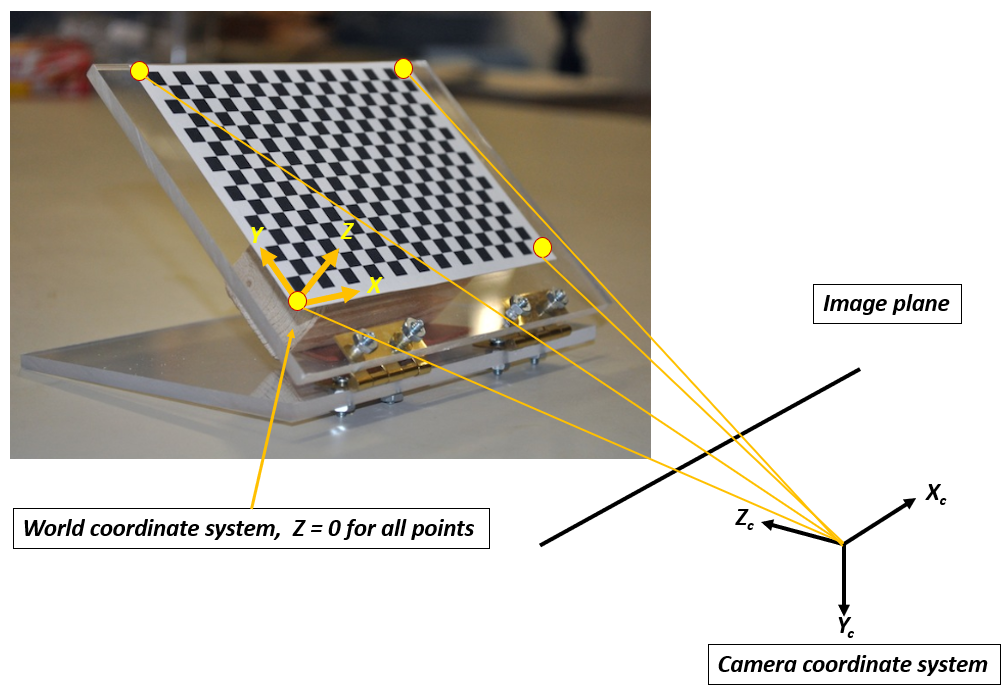
\includegraphics[width=\linewidth]{2D_2D.png}
	\caption{Mapping 2D planar world points (Z = 0) on to a 2D image plane.}
	\label{fig:2D_3D}
\end{figure}

The disadvantage of 2D/3D correspondence way of estimating the projection matrix is that complete knowledge of the 3D location has to be known and it has to be precise as well. There is a flexible and computationally easy method to estimate the projection matrix thereby intrinsic and extrinsic camera parameters, developed by Zhang \cite{Zhang} using a 2D planar object in 3D space as shown in \cref{fig:2D_3D} along with its 2D image. Let us recall the equation \ref{eq:mat_pixel_t_world} 

\begin{equation*}
Z_c \left[ 
\begin{array}{c} u\\ v\\ 1 \end{array} 
\right] = 
\begin{bmatrix}
\alpha_x & S & C_x \\
0 & \alpha_y & C_y \\
0 & 0 & 1
\end{bmatrix} 
\begin{bmatrix}
r_{11} &r_{12}  &r_{13}  &t_x\\
r_{21} &r_{22}  &r_{23}  &t_y\\
r_{31} &r_{32}  &r_{33}  &t_z \\
0 &0  &0  &1
\end{bmatrix}
\left[ 
\begin{array}{c} X\\ Y\\ Z\\ 1 \end{array} 
\right]
\end{equation*}

Using 2D planar object we eliminate Z coordinate thereby eliminating $3^{rd}$ column of the extrinsic matrix.

\begin{equation*}
Z_c \left[ 
\begin{array}{c} u\\ v\\ 1 \end{array} 
\right] = 
\begin{bmatrix}
\alpha_x & S & C_x \\
0 & \alpha_y & C_y \\
0 & 0 & 1
\end{bmatrix} 
\begin{bmatrix}
r_{11} &r_{12}  &r_{13}  &t_x\\
r_{21} &r_{22}  &r_{23}  &t_y\\
r_{31} &r_{32}  &r_{33}  &t_z \\
0 &0  &0  &1
\end{bmatrix}
\left[ 
\begin{array}{c} X\\ Y\\ 0\\ 1 \end{array} 
\right]
\end{equation*}

\begin{equation}
Z_c \left[ 
\begin{array}{c} u\\ v\\ 1 \end{array} 
\right] = 
\begin{bmatrix}
\alpha_x & S & C_x \\
0 & \alpha_y & C_y \\
0 & 0 & 1
\end{bmatrix} 
\begin{bmatrix}
r_{11} &r_{12}  &t_x\\
r_{21} &r_{22}  &t_y\\
r_{31} &r_{32}  &t_z \\
0 &0 &1
\end{bmatrix}
\left[ 
\begin{array}{c} X\\ Y\\ 1 \end{array} 
\right]
\label{eq:mat_2D_pixel_t_world}
\end{equation}

As in the case of 2D/3D problem setup, The equation \ref{eq:mat_2D_pixel_t_world} can be compactly written by combining both intrinsic and extrinsic matrices known an Homography matrix \textbf{$H_{3\times3}$}. And $\lambda$ is a arbitrary scaling factor for which equation \ref{eq:mat_homography} is satisfied. In other words, A projection matrix \textbf{$P_{3\times4}$} in planar case reduces to homography matrix \textbf{$H_{3\times3}$}.

\begin{equation}
\lambda \left[ 
\begin{array}{c} u\\ v\\ 1 \end{array} 
\right] = 
\begin{bmatrix}
h_{11} &h_{12}  &h_{13} \\
h_{21} &h_{22}  &h_{23} \\
h_{31} &h_{32}  &h_{33} \\
\end{bmatrix}
\left[ 
\begin{array}{c} X\\ Y\\ 1 \end{array} 
\right]
\label{eq:mat_homography}
\end{equation} 

As in the case of 2D/3D problem, the homography matrix H will be estimated using a given set of 2D planar world points and 2D image points and then it will be decomposed to intrinsic and extrinsic matrices.\\

Given a set of N corresponding 2D/2D points (\textbf{$u_i$},\textbf{$X_i$}), a homography matrix H is needed such that
\begin{equation*}
	\lambda\textbf{$u_i$} = H \textbf{$X_i$}\ ,  where\ i = 1......N
\end{equation*}
Problem set up in 2D/2D case is very similar to 2D/3D problem except that the homography matrix has 9 non-trivial elements thus 8 degrees of freedom (ignoring scaling) therefore 8 independent equations are necessary to estimate H, hence 4 2D/2D point correspondences are required. At this point, the same estimating procedure used previously can be employed.\\

\textbf{Exact solution.} With a minimum of 4 correspondences, the solution to $Ah = 0 $ will be exact which means 2D world points will be exactly gets projected to their measured image points correspondingly. The exact solution h, to Ah = 0 is the right nullspace of matrix A.\\

\textbf{Over-determined solution.} In this case solution to Ah = 0 will be obtained by minimizing the algebraic or geometric error of projection, subjected to some valid constraints.\\ 

\textbf{Minimizing algebraic error.} In this case the approach is,   

\begin{equation}
\begin{matrix}
\displaystyle \min & ||Ah|| & \textrm{s.t.} & ||h|| = 1\\
\end{matrix}
\label{eq:min_2D_algebraic}
\end{equation}
The solution to \cref{eq:min_2D_algebraic} is obtained from unit singular value of A corresponding to the smallest singular value (the least square problem of type II, see appendix).\\

\textbf{Minimizing geometric error} The geometric error in the image in 2D/2D case is
\begin{equation*}
\begin{matrix}
\displaystyle \sum_{i=1}^{n} d (u_i, \hat{u}_i)^2 
\end{matrix}
\end{equation*}
where $u_i$ is measured point in image and $\hat{u}_i$ is H \textbf{$X_i$} which is the exact projrction of \textbf{$X_i$} on to the image under H. If the measurement errors are Gaussian then the solution to 
\begin{equation}
\begin{matrix}
\displaystyle \min_{P} \sum_{i=1}^{n} d (u_i, H\textbf{$X_i$})^2 
\end{matrix}
\label{eq:min_geometric}
\end{equation}
is the maximum likelihood of H. Minimizing geometric error requires non-linear iterative methods such as Levenberg-Marquardt (LM) algorithms. Local minima can be found via LM, in order to find the global minima, initial starting point can be linear soution obtained from \ref{eq:min_algebraic}.\\

The disadvantage of 2D/2D homography is that with a single homography, not all the parameters of a projection matrix can be determined as Z coordinate of the world point is eliminated.  
\begin{equation*}
\textbf{H} = \begin{bmatrix}
\textbf{p}_{1} & \textbf{p}_{2}  & \textbf{p}_{4} \\
\end{bmatrix}
\end{equation*} 
The decomposition of H to obtain extrinsic and intrinsic matrices is not possible, therefore, follows a different approach. We will first see how to get the intrinsic matrix K and as soon we have K, obtaining extrinsic is trivial.\\

\textbf{Intrinsics} Recall that $H = K\ [\textbf{r}_1\  \textbf{r}_2\  \textbf{t}] = [\textbf{p}_1\ \textbf{p}_2\ \textbf{p}_3]$ and the fact that R is a rotational matrix and can be expressed as,

\begin{equation*}
\begin{split}
\mathbf{r}_1^\intercal \mathbf{r}_2  = 0\\ 
\mathbf{r}_1^\intercal \mathbf{r}_1  = \mathbf{r}_2^\intercal \mathbf{r}_2  = 1 
\end{split}	
\end{equation*}
rewriting with K gives,
\begin{equation*}
\begin{split}
\mathbf{p}_1^T K^{-T} K^{-1} \mathbf{p}_2 = 0 \\
\mathbf{p}_1^T K^{-T} K^{-1} \mathbf{p}_1 = \mathbf{p}_2^T K^{-T} K^{-1} \mathbf{p}_2   = 1
\end{split}	
\end{equation*}
defining $\textbf{$\omega$}$ = $K^{-T} K^{-1}$ as a symmetric matrix, above equations can be written as,
\begin{equation*}
\omega = 
\begin{bmatrix}
\omega_{11} &\omega_{12}  &\omega_{13} \\
\omega_{12} &\omega_{22}  &\omega_{23} \\
\omega_{13} &\omega_{23}  &\omega_{33} \\
\end{bmatrix}
\end{equation*} 
\begin{equation}
\begin{split}
\mathbf{p}_1^T \omega \mathbf{p}_2 = 0 \\
\mathbf{p}_1^T \omega \mathbf{p}_1 - \mathbf{p}_2^T \omega \mathbf{p}_2  = 0
\end{split}	
\label{eq:intrinsic}
\end{equation}

$\textbf{p}_1$ and $\textbf{p}_2$ are known from homography matrix and $\vect{\omega}$ has to be calculated. $\vect{\omega}$  can be estimated with techniques that we employed earlier with DLT and SVD by defining $ \textbf{b} = (\omega_{11}\ \omega_{12}\ \omega_{13}\  \omega_{22}\ \omega_{23}\ \omega_{33})^T $ and solving $ \textbf{A} \textbf{b} = 0.$ Each homography provides 2 independent rows therfore 3 such homographies are required to estimate $\vect{\omega}$ . Once the $\vect{\omega}$  is computed it can be decomposed in to $K^{-T} K^{-1}$ using Cholesky decomposition.\\

\textbf{Extrinsics.} Computing extrinsics post intrinsics is very straight forward as given by \cite{Zhang} we will first calculate rotation matrix followed by translation vector. $H = K\ [\textbf{r}_1\  \textbf{r}_2\  \textbf{t}] $ having known K we can rearrange as $\inv{K}\ H = H^{'} =  [\textbf{h}_1^{'}\  \textbf{h}_2^{'}\  \textbf{h}_3^{'}] $ which is theoritically equal to $[\textbf{r}_1\  \textbf{r}_2\  \textbf{t}] $. Since the rotational matrix is a orthogonal matrix, third column is othogonal to first 2 and therefore can be calculated by vector cross product $ [\textbf{h}_1^{'} \times \textbf{h}_2^{'} ] $ hence, the complete rotational matrix is  $ Q = [\textbf{h}_1^{'}\ \textbf{h}_2^{'}\ \textbf{h}_1^{'} \times\ \textbf{h}_2^{'} ] $ again which is theoritically equal to $ R = [\textbf{r}_1\ \textbf{r}_2\ \textbf{r}_1\ \times\ \textbf{r}_2\ ] $ which may not be true due to the noisy data. Therefore,  it necessary to find a best 3x3 rotation matrix  R from a given 3x3 matrix Q, here "best" in the sense of smallest Frobenius norm of the difference $[R-Q]$ (see appendix). If the SVD of given matrix is $ Q = UDV^T $, then the best rotation matrix is given by $UV^T$. The translation vector can be calculated as  $ \textbf{t} = \textbf{h}_3^{'}$ but the vector $\textbf{t} $ has to be normalised therefore $\textbf{t} = \textbf{h}_3^{'} / \|\textbf{h}_1^{'}\|$.

\subsection{Lens distortions} A world point is mapped to image plane as \( (x, y, z)^T \) = \( (\textit{f}\frac{X_c}{Z_c}, \textit{f}\frac{Y_c}{Z_c}, \textit{f} )^T\) then image points are mapped to pixel coordinates as \( (u, v, z)^T \) = \( ( x+C_x, y+C_y, \textit{f} )^T \) however, usually, there are radial and tangential distortions in the lens as depicted in \cref{fig:distortion} therefore, image coordinates have to be corrected before mapping to pixel coordinates. The corrected image coordinates are

\begin{equation}
\begin{split}
x^{'} = x \times \frac{1+k_1r^2+k_2r^4+k_3r^6}{1+k_4r^2+k_5r^4+k_6r^6} + 2p_1xy + p_2(r^2+2x^2)\\
y^{'} = y \times \frac{1+k_1r^2+k_2r^4+k_3r^6}{1+k_4r^2+k_5r^4+k_6r^6} + p_1(r^2+2y^2) + 2p_2xy\\ 
\end{split}	
\label{eq:lens_distortion}
\end{equation}

\noindent where $ r^2 = (x^2+y^2) $ , $ k_1 .....k_6 $ are the radial distortion coefficients and  $ p_1, p_2 $ are the tangential distortion coefficients. It is these corrected image coordinates are mapped to pixel coordinates as \( (u, v, z)^T \) = \( ( x^{'} +C_x, y^{'} +C_y, \textit{f} )^T \).

\begin{figure}[hbt!]
	\centering
	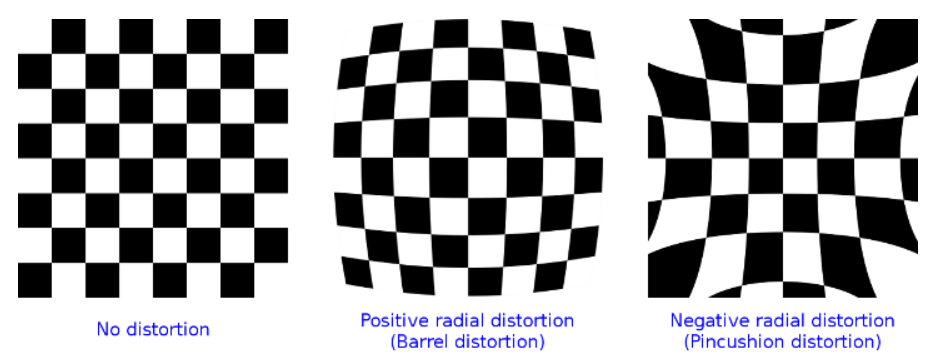
\includegraphics[width=\linewidth]{distortion.png}
	\caption{Barrel distortion $(typically \ k_1 > 0 )$ and pincushion distortion $(typically k_1 < 0)$ \cite{OpenCV}} 
	\label{fig:distortion}
\end{figure}
\newpage
Camera calibration is the process of determining, intrinsic, extrinsic parameters along with distortion coefficients. The \cref{tab:Calibration_summary_table} summarizes the calibration process discussed above. 

\begin{table}[hbt!]
	\centering
	\begin{tabular}{|cccccc|}
		\hline
		correspondences & Min. points & No.of images & [R\ |\ t] & K & world points\\ 
		\hline
		2D im./3D world & $\geq$ 6 & 1 & \checkmark & \checkmark & given \\
		2D im./2D world & $\geq$ 4 & 3 & \checkmark & \checkmark  & given \\
		2D im./2D world & $\geq$ 4 & 1 & \checkmark  & given & given \\
		\hline
	\end{tabular}
	\caption{Calibration summary table}
	\label{tab:Calibration_summary_table}
\end{table}

\section{Camera calibration and pose estimation}
Camera calibration is carried out using open-source computer vision library OpenCV \cite{OpenCV}. Camera calibration is based on 2D/2D point correspondences with the chessboard as a 2D planar object. The homography is calculated using square corners of a chessboard (world points) and its image points. OpenCV needs an arrays of world points and image points and the grid size of the chessboard (in our case its 5 rows, 8 columns). Therefore, 10 RGB images of the chessboard at different position and orientation was recorded and an array of world points (x,y) location of chessboard corners [(0,0), (40,0), (80,0)...] was fed to the algorithm. OpenCV automatically detects these chessboard corners from the images as shown in \cref{fig:chessboard_corners} and refines them accordingly.

\begin{figure}[hbt!]
	\centering
	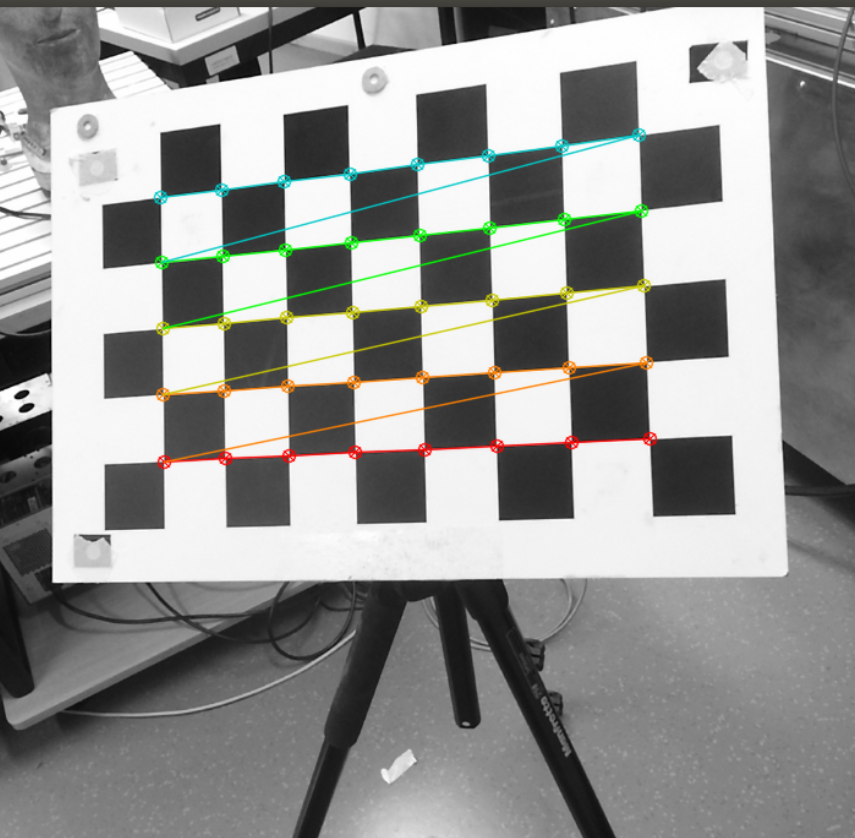
\includegraphics[scale=0.6]{chessboard_corners.png}
	\caption{Chessboard corners(image points) detection in OpenCV}
	\label{fig:chessboard_corners}
\end{figure}

\begingroup\makeatletter\def\@currenvir{verbatim}
\verbatim
cv2.calibrateCamera(object_points, image_points, ...)
output: rms, camera_matrix, dist_coeffs, rot_vecs, trans_vecs
\end{verbatim}

The OpenCV function cv2.calibrateCamera takes in these world points (object points), image points and some more arguements then outputs geometric error of reprojection (rms), intrinsic parameters (camera\_matrix) distortion coefficients (dist\_coeffs) and extrinsic parameters $(rot\_vecs, trans\_vecs)$.

Having completed the camera calibration we can now make use of the intrinsic parameters and the distortion coefficients as an input to the pose estimation algorithm provided by OpenCV. 

\begingroup\makeatletter\def\@currenvir{verbatim}
\verbatim
cv2.solvePnP(object_points, image_points, intr_mat, dist_coeffs)
output: rot_vecs, trans_vecs 
\end{verbatim}


The OpenCV function cv2.solvePnP takes object points, image points, intrinsic matrix, and distortion coeffcients as the arguments and computes rotation and translation vectors. Rotation vector can be converted to 3$\times$3 rotational matrix using cv2.Rodrigues function provided by openCV. By combining rotation matrix and translation vector we can form 4$\times$4 homogenious matrix for further manipulation.